\documentclass[11pt]{article}
\usepackage{amsmath, amssymb, amsthm}
\usepackage{geometry}
\usepackage{graphicx}
\geometry{margin=1in}
\setlength\parindent{0pt}
\title{Foundations of Machine Learning -- Lecture 6 Notes}
\author{}
\date{}

\begin{document}
\maketitle

\section*{Generative Adversarial Networks}

Generative Adversarial Network, is a type of machine learning model used for generating new data that resembles a given dataset — such as creating realistic images, music, or text.
The core idea is that it consists of two neural networks trained together in a game-like setup:
\begin{itemize}
	\item Generator (G): creates fake data trying to mimic real data (e.g., fake images).
	\item Discriminator (D): evaluates data and tries to tell if it’s real (from the training data) or fake (from the generator).
\end{itemize}

\begin{figure}[h]
	\centering
	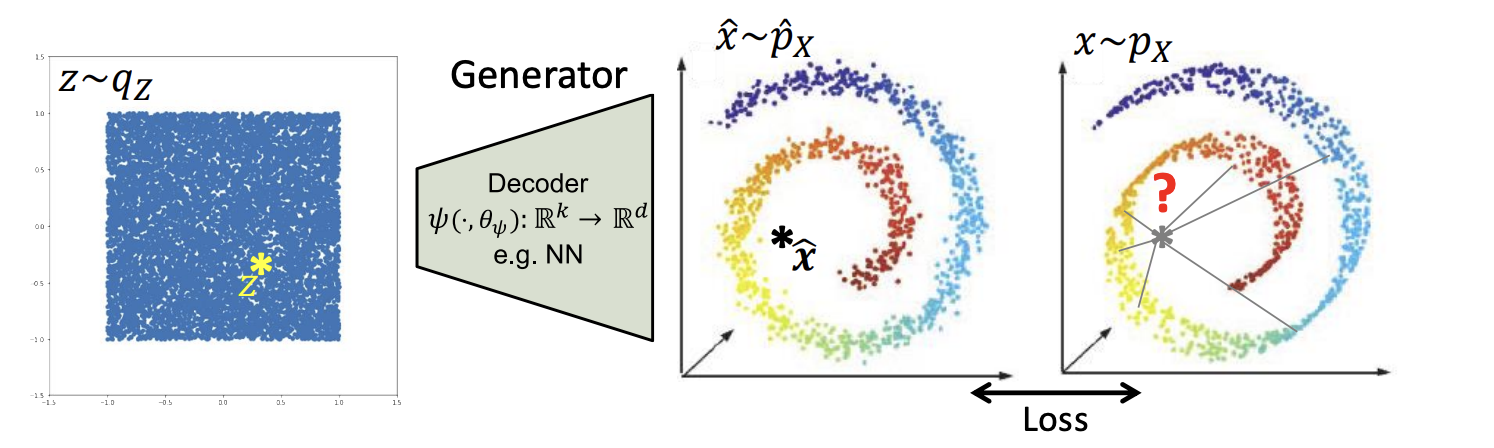
\includegraphics[width=0.9\textwidth]{../imgs/gan_img.png} % 
\end{figure}

We want to use an adversarial network that tries to distinguish points on the manifold of the real data
from any other points in $\mathbb{R}^d$.

\medskip

Let $\eta(x; \theta_\eta): \mathbb{R}^d \rightarrow [0, 1]$ be the \textbf{discriminator}.

and $\hat{x}_j = \psi(z_j; \theta_\psi)$ be the \textbf{Generator}.

\medskip

Then the GAN objective is given by

\[
	\min_{\theta_\psi} \max_{\theta_\eta}
	\left[
		\frac{1}{N} \sum_i \log \big( \eta(x_i; \theta_\eta) \big)
		+
		\frac{1}{M} \sum_j \log \big( 1 - \eta(\hat{x}_j; \theta_\eta) \big)
		\right],
\]

The discriminator wants the first term to be large (as that means it correctly identifies real as real)
and the last term to also be large (as it means it correctly identifies fake from fake)
\medskip
The generator cant change the first term, but wants the second term to be small as that means it fooled the discriminator into identifying a fake as real.

\pagebreak

\begin{figure}[h]
	\centering
	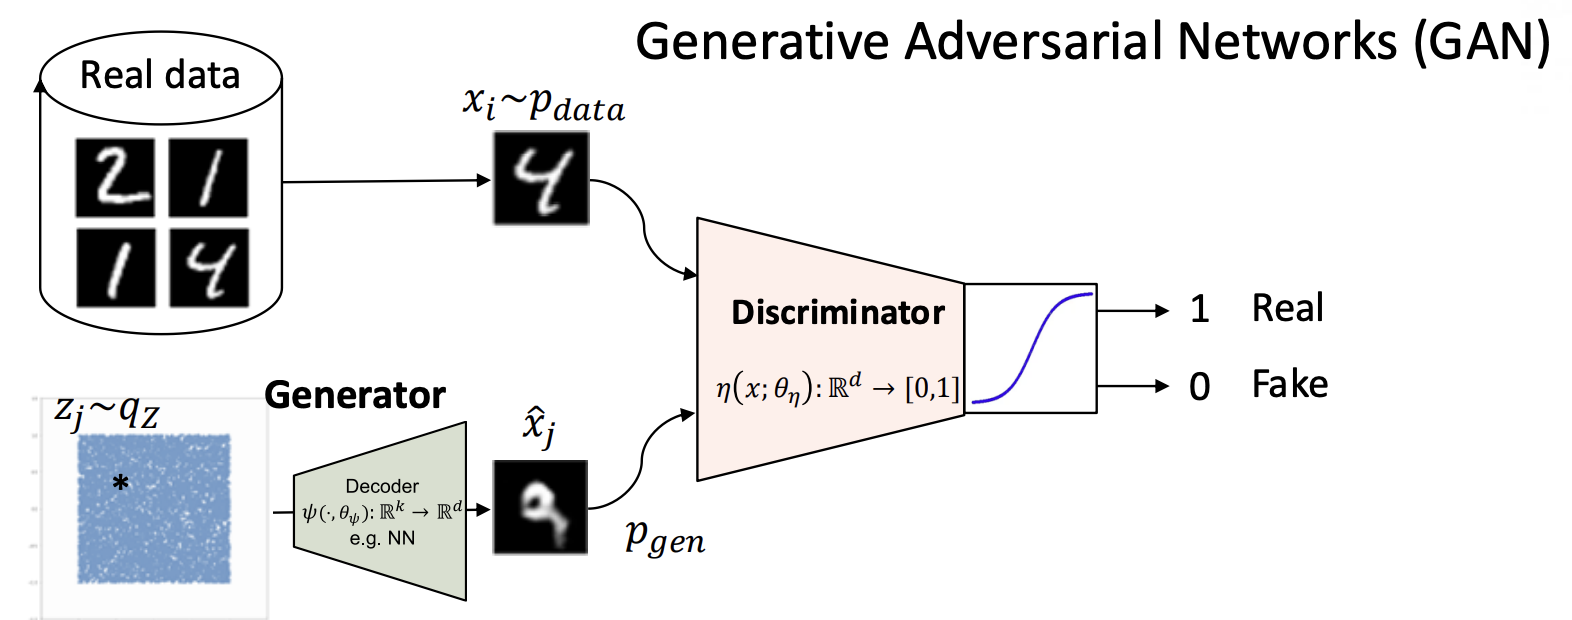
\includegraphics[width=0.9\textwidth]{../imgs/gan-optimization.png} % 
\end{figure}


If maximization over $\theta_\eta$ is performed and we obtain the optimal discriminator,
the original min--max problem reduces to:

\[
	\min_{\theta_\psi} JS(p_{\text{data}} \,\|\, p_{\text{gen}})
\]

where $JS(\cdot \| \cdot)$ denotes the \textbf{Jensen--Shannon divergence}, defined as:

\[
	JS(p \,\|\, q) = \tfrac{1}{2} KL\!\left(p \,\Big\|\, \tfrac{p + q}{2}\right)
	+ \tfrac{1}{2} KL\!\left(q \,\Big\|\, \tfrac{p + q}{2}\right)
\]

\begin{itemize}
	\item The Jensen--Shannon divergence measures the distance between two probability distributions.
	\item When $JS(p_{\text{data}} \,\|\, p_{\text{gen}}) = 0$, the two distributions are identical.
	\item Minimization over $\theta_\psi$ means choosing the $p_{\text{gen}}$ that is closest to the target distribution $p_{\text{data}}$.
\end{itemize}


\subsection*{GAN's Formulation}

The training of a Generative Adversarial Network (GAN) is formulated as a \textbf{minimax game} between two networks:
a \textbf{discriminator} $D$ and a \textbf{generator} $G$.

\[
	\min_G \max_D V(D, G)
\]

The value function $V(D, G)$ is defined as:
\[
	V(D, G) =
	\mathbb{E}_{x \sim p(x)} [\log D(x)] +
	\mathbb{E}_{z \sim q(z)} [\log(1 - D(G(z)))].
\]

\begin{itemize}
	\item $\mathbb{E}_{x \sim p(x)}[\log D(x)]$: expectation over real samples.
	      Rewards the discriminator for assigning high probabilities to real data.
	\item $\mathbb{E}_{z \sim q(z)}[\log(1 - D(G(z)))]$: expectation over generated (fake) samples.
	      Rewards the discriminator for correctly identifying fake data as fake.
\end{itemize}

\pagebreak

Game dynamics:
\begin{itemize}
	\item The discriminator $D$ tries to \textbf{maximize} $V(D, G)$ — it wants to correctly classify real vs. fake samples.
	\item The generator $G$ tries to \textbf{minimize} $V(D, G)$ — it wants to fool the discriminator into classifying generated data as real.
\end{itemize}

At Nash equilibrium:
\[
	p_{\text{data}}(x) = p_{\text{gen}}(x), \quad \forall x,
\]
\[
	D(x) = \frac{1}{2}, \quad \forall x.
\]

At this point, the discriminator cannot distinguish between real and generated samples,
and the generator has learned to reproduce the true data distribution.

\subsection*{GAN Algorithm:}
Given a number of training iterations $N$ and number of discriminator updates per iteration $k$.

\begin{enumerate}
	\item \textbf{For each training iteration:}
	      \begin{enumerate}
		      \item \textbf{Discriminator updates (repeated $k$ times):}
		            \begin{itemize}
			            \item Sample a minibatch of $m$ noise samples $\{ z^{(1)}, \ldots, z^{(m)} \}$ from noise prior $p_g(z)$.
			            \item Sample a minibatch of $m$ real examples $\{ x^{(1)}, \ldots, x^{(m)} \}$ from data distribution $p_{\text{data}}(x)$.
			            \item Update the discriminator by ascending its stochastic gradient:
			                  \[
				                  \nabla_{\theta_d} \frac{1}{m} \sum_{i=1}^{m}
				                  \Big[
					                  \log D(x^{(i)}) + \log \big(1 - D(G(z^{(i)}))\big)
					                  \Big].
			                  \]
		            \end{itemize}

		      \item \textbf{Generator update:}
		            \begin{itemize}
			            \item Sample a minibatch of $m$ noise samples $\{ z^{(1)}, \ldots, z^{(m)} \}$ from noise prior $p_g(z)$.
			            \item Update the generator by descending its stochastic gradient:
			                  \[
				                  \nabla_{\theta_g} \frac{1}{m} \sum_{i=1}^{m}
				                  \log \big(1 - D(G(z^{(i)}))\big).
			                  \]
		            \end{itemize}
	      \end{enumerate}
\end{enumerate}

\subsection*{Problems with GANs}
\paragraph*{Non-convergence in GAN Training}

Learning models (in general) involve a single player. The player tries to maximize its reward (or equivalently, minimize its loss). And Gradient Descent (GD) is used to find the optimal parameters.
With non-convex loss functions, we might converge only to local optima.

\medskip

GANs instead involve two (or more) players:
\begin{itemize}
	\item The Discriminator ($D$) is trying to \textbf{maximize} its reward.
	\item The Generator ($G$) is trying to \textbf{minimize} the Discriminator's reward.
\end{itemize}

\[
	\min_G \max_D V(D, G)
\]

Traditional gradient descent does not guarantee convergence in such adversarial settings,
so the generator and discriminator may oscillate, diverge, or collapse instead of stabilizing.

\paragraph*{Mode Collapse}
Mode collapse happens when the generator stops producing diverse outputs and instead maps many different noise inputs $z$ to the same or very similar outputs.

Formally, instead of learning a distribution $p_{\text{gen}}(x)$ that matches the true data distribution $p_{\text{data}}(x)$, 
the generator collapses to a few modes (or even a single mode).


\end{document}

